\chapter{Metodologia} \label{Metodologia}


\section{Tecnologias Utilizadas} \label{tecnologiasUtilizadas}

    Para a implementação deste trabalho, foi utilizada a biblioteca OpenCV, versão 2.4.8. Essa biblioteca desenvolvida pela Intel dá acesso a várias funções importantes para Processamento de imagens e Visão computacional em diversas linguagens como C++, Python e Java. Nesse trabalho a linguagem escolhida foi o C++. Foi escolhida a versão 2.4.8 ao invés da mais recente 3.0.0 pela sua consistência e facilidade de instalação, além de uma documentação mais completa.
    
    A IDE utilizada foi a Microsoft Visual Studio 2015 versão Community. Essa IDE foi escolhida por causa da grande facilidade que traz para a instalação de bibliotecas externas como a OpenCV utilizada no trabalho e também por causa da possibilidade de se instalar diversos plugins que podem facilitar o desenvolvimento, como o Image Watch, plugin que permite a visualização das imagens geradas pelo programa em grande detalhe.

%Seçao sobre como obti as imagens para os testes do trabalho ---- a maquete/o drone.




\section{Segmentação dos veículos} \label{segmentacaoVeiculos}

    A primeira etapa na implementação do programa apresentado nesse trabalho é a da segmentação dos veículos em movimento durante o decorrer do vídeo obtido pela câmera estática. Para detectar esse veículos, esse projeto utiliza uma técnica de segmentação baseada naquela apresentada em \cite{hai2009self}. Segmentar corretamente os carros é crucial para o procedimento descrito na seção \ref{geracaoFundo}. Nessa seção, descrevo como uma imagem com apenas o contorno de um carro é obtida.

    Primeiramente, é extraída a imagem de diferença entre dois quadros consecutivos. Chamamos essa imagem de \textit{D}. Essa diferença é trivial, nada mais é do que o valor absoluto da diferença entre o valor do mesmo \textit{pixel} em cada um dos dois quadros. Pixels que representam objetos que se mantiveram estáticos durante os dois quadros originais, como o asfalto e carros estacionados, devem ter então valor zero em \textit{D}. Portanto, é de se esperar que a imagem \textit{D} tenha uma grande quantidade de valores próximos ou iguais a zero.

    Após extraída a diferença entre os dois quadros, resta binarizar \textit{D}. Como descrito na seção \ref{segmentacao}, é preciso encontrar um limiar apropriado para cada imagem de diferença obtida. Como elas são obtidas dinamicamente, determinar esse limiar de forma estática, não traz resultados satisfatórios. Pares de quadros que apresentam menos movimento possuem valores de diferença menores e portanto, as regiões que devem ser tornadas brances têm valores inicialmente mais baixos.

    Sabendo que a grande maioria dos pixels de \textit{D} possui valor próximo a zero, podemos determinar um limiar \textit{T} de forma dinâmica. Para encontrar o valor ideal de \textit{T}, o programa primeiro encontra o pico do histograma de \textit{D}. O nível de cinza correspondente a esse valor é o que mais ocorre na imagem e será sempre um valor bem próximo de zero. O valor escolhido para \textit{T} é o terceiro nível de cinza cujo valor no histograma é inferior a 1\% do valor do pico. A escolha desse valor ao invés do primeiro vem de um problema gerado por ruído na captura da imagem.

    Por conta de ruído na imagem, valores de pixels em pontos estáticos, como por exemplo, parte do asfalto, apresentam pequenas diferenças que poluem a imagem de diferença. Esses pequenos pontos com difereça maior que zero podem aparecer na imagem binarizada, gerando regiões indesejadas. Para minimizar esse problema, duas medidas são tomadas. A primeira é a aplicação do parâmetro do limiar mínimo \textit{lm}. Esse valor depende do vídeo sendo analizado e deve ser maior quanto maior for o ruído da câmera. Antes do cálculo do histograma da imagem de diferença o programa configura todos os valores abaixo desse limiar para o valor mínimo. Isso desvia o histograma para valores menores e gera uma binarização mais limpa. A determinação correta de \textit{lm} é essencial para uma boa segmentação. A segunda medida é a escolha do terceiro valor inferior a 1\% do pico. Isso evita apenas que o ruído não seja responsável ao acaso pelo limiar escolhido estar abaixo do desejado. A figura \ref{fig:Diferenca} mostra o resultado do processo.

    \begin{figure}[h]
      \centering
      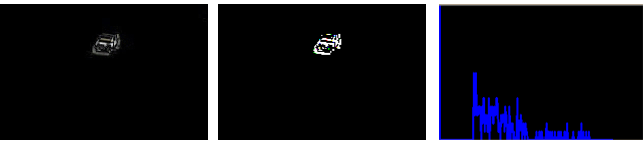
\includegraphics[width=\textwidth]{FiguraDiferenca}
      \caption{A esquerda: a imagem de diferença D. Ao centro: D binarizada com a técnica descrita acima. A direita: o histograma de D}\label{fig:Diferenca}
    \end{figure}

\section{Rastreamento dos veículos} \label{rastreamentoVeiculos}
    
      A técnica de segmentação de veículos apresentada na seção \ref{segmentacaoVeiculos} provê resultados parciais que podem ser utilizados e processados para se atingir obter diversas informações. Uma possibilidade é a geração de fundo dinâmica apresentada na seção \ref{geracaoFundo}. O outro tratamento que esse programa dá para as imagens obtidas na seção \ref{segmentacaoVeiculos} é rastrear os objetos que estão em movimento no vídeo através do acompanhamento das diferenças entre quadros.
      
      Para cada imagem $D$ binária obtida quando se faz a diferença entre dois quadros do vídeos, o programa procura os contornos de todas as manchas brancas presentes na imagem e os armazena em um vetor. Em seguida, o progrma calcula o menor círculo que contém completamente cada um desses contornos e armazena os seus centros em um vetor $C$ de coordenadas.
      
      O programa possui ainda uma estrutura de Rastro, que possui duas coordenadas: a do início e o fim do rastro. Uma vetor $R$ de rastros armazena cada rastro que está ainda sendo computado pelo programa.
      
      Munido de $R$, $C$ e a imagem $D$ gerada pela diferença entre os quadros, o programa passa a analisar de quais rastros cada centro faz parte. Ele percorre o vetor de $C$ de centros dos contornos e o compara com as coordenadas dos finais de cada rastro em $R$. Se $R$ estiver vazio, um novo rastro é criado com início no centro que está sendo analisado e final provisoriamente populado com o valor de coordenada igual ao do ínicio. Caso contrário, o programa verifica se o centro analisado $c$ atende as seguintes condições em relação ao final de um determinado rasto $f_{R}$:
      
      \begin{itemize}
        \item Distância Máxima: A coordenada de $c$ a uma distância menor da coordenada de $f_{R}$ do que uma distância máxima determinada manualmente. Essa distância é calculada utilizando um método de distância euclidiana simples, apresentado na equação \ref{distanciaEuclidiana}. Se $c$ não cumpre essa condição, o programa considera imediatamente que ele não deve fazer parte da rastro em questão.
        \item Ângulo entre vetores: Para evitar que um veículo que passa muito próximo a outro em sentido oposto "tome conta" do seu rastro, o ângulo vetorial entre $c$ e $f_{R}$ é calculado. Novamente, ele não pode ultrapassar um limiar imposto manualmente.
        \item Direção predominante das bordas: Os contornos em $D$ possuem bordas que podem ser analisadas para determinar direção, usando uma multiplicação matricial que se assemelha a operação da derivada. Essa terceira condição tem o papel apenas de complementar a segunda.
      \end{itemize}
      
      Se $c$ atende às condições listadas acima para o final de algum rastro, $c$ passa a ser o final daquele rastro e o programa passa para o próximo contorno a ser analisado.
      
      Se o final de um rastro não sofrer mudanças significativas por um certo intervalo de tempo, ele é determinado como um rastro finalizado. Nesse momento, o programa verifica o ponto de início e o ponto do fim desse rastro. Se ele iniciou em um ponto exterior a uma vaga e  finalizou em um ponto interior, o algoritmo então marca que essa vaga foi possivelmente ocupada. Essa marcação serve como validação para as diferenças encontradas na seção \ref{verificaoObjetosFundo}.
      
      \begin{equation}\label{distanciaEuclidiana}
        (a,b) - (c,d) = \sqrt{(a-c)^2 + (b-d)^2}
        \caption{A equação da distância euclidiana entre os pontos (a,b) e (c,d)}
      \end{equation}
      
      A cada quadro, o programa utiliza essas informações para desenhar círculos nas posições que cada rastro ocupou em uma outra imagem que contém apenas o fundo da imagem do vídeo e os círculos dos rastros. Cada rastro tem uma cor associada. A figura \ref{rastrosFig} mostra um desses rastros e o momento do início e final dele.
      
      \begin{figure}
 \centering
\begin{subfigure}{.5\textwidth}
  \centering
  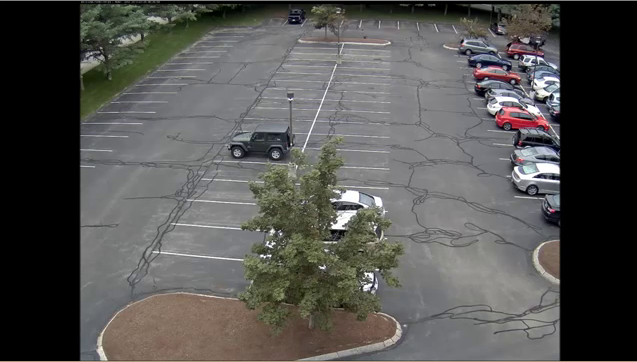
\includegraphics[width=.8\linewidth]{MomentoRastro1}
  \caption{}
  \label{rastrosFig:sfig1}
\end{subfigure}\


\begin{subfigure}{.5\textwidth}
  \centering
  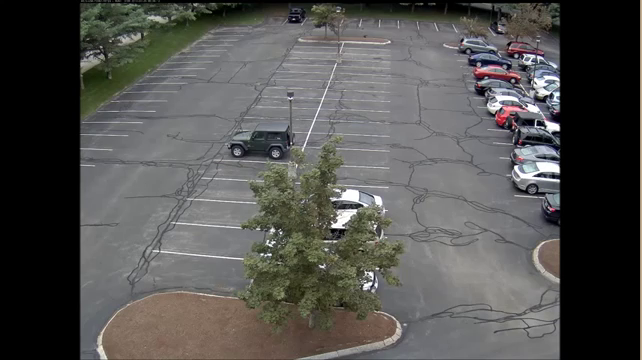
\includegraphics[width=.8\linewidth]{MomentoRastro2}
  \caption{}
  \label{rastrosFig:sfig2}
\end{subfigure}


\begin{subfigure}{.5\textwidth}
  \centering
  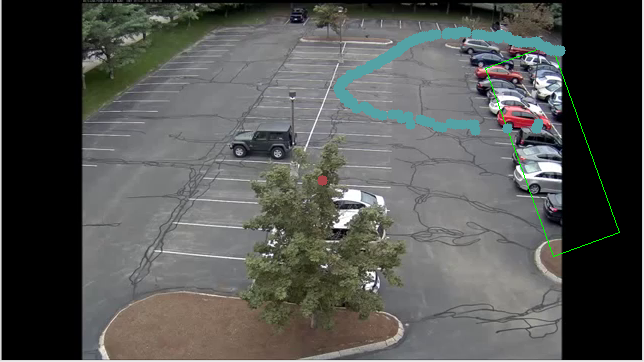
\includegraphics[width=.8\linewidth]{Rastro}
  \caption{}
  \label{rastrosFig:sfig2}
\end{subfigure}
\caption{(a) Um carro aparecendo na cena ; (b)O mesmo carro estacionado em uma vaga; (c) O rastro gerado pelo programa}
\label{rastrosFig}
\end{figure}
      
      
      





\section{Geração de Fundo Dinâmico} \label{geracaoFundo}

     Uma etapa importante do trabalho é a geração de uma imagem de fundo, separada da imagem do vídeo original. Para tal, é preciso implementar um método que separe os elementos do \textit{background} daqueles do \textit{foreground}. Determinamos que os elementos do fundo são aqueles que não estão se movimentando no momento, enquanto os elementos do \textit{foreground} são os objetos que se movem na imagem, em particular, os carros. É importante construir essa imagem, pois é essa segmentação de fundo e plano principal que permitirá mais tarde que o programa determine se uma vaga foi ocupada ou desocupada por um veículo.

     Gerar essa imagem de fundo não é uma tarefa trivial. Devido a própria natureza do espaço sendo filmado, veículos que antes compunham o fundo da imagem podem passar a se mover e veículos que estão em movimento em um determinado momento eventualmente vão estacionar e devem passar a integrar o \textit{background}. É preciso então ter muito cuidado na determinação do fundo do vídeo.

     Antes de mais nada, é preciso determinar uma imagem de fundo inicial. Esse fundo inicial será usado pelo processo de geração dinâmica de fundo descrito mais abaixo. A imagem de fundo base é construída no momento da instalação do \textit{software} deste trabalho, e pode ser reconstruída sempre que desejado, como no início do dia ou no horário que as atividades do estacionamento se iniciam.

     A imagem de fundo inicial \textit{Fi} é formada usando os 30 primeiros quadros capturados em vídeo a partir do momento que sua formação se inicia. O valor de cada \textit{pixel} \textit{i} na imagem tem valor igual a média do valor desse \textit{pixel} em cada um desses quadros, calculada por:

     \begin{equation}\label{mediaFundoInicial}
       V_{i} = \frac{1}{30}\sum_{t=1}^{30}V_{it}
     \end{equation}

     Onde $V_{i}$ é o valor do \textit{pixel} \textit{i} em \textit{Fi} e $V_{it}$ é o valor do \textit{pixel} \textit{i} no frame de número \textit{t}.

     Uma vez obtida \textit{Fi} não podemos simplesmente utilizá-la como um fundo definitivo. A determinação do \textit{background} deve ser feita de forma dinâmica e constante por conta de diversos fatores. Alguns deles são:

     \begin{itemize}
       \item Mudanças na iluminação: com o passar do dia, tanto a iluminação natural quanto a artificial sofrem mudanças. Essas alterações podem fazer com que a cor do asfalto percebida pela câmera mude. É importante adaptar o fundo para que isso não surja como uma diferença entre dois quadros consecutivos
       \item Comportamente dos carros: veículos anteriormente parados podem começar a se mover e veículos em movimento vão estacionar. É preciso adaptar o \textit{background} a esses eventos.
       \item Ruído da câmera: um fundo adaptativo e dinâmico minimiza os problemas causados por ruído na captação do vídeo.
     \end{itemize}

     Para atualizar corretamente o fundo do vídeo, precisamos primeiramente determinar a região do \textit{foreground} da imagem. Para tal, o programa utiliza a imagem D obtida na seção \ref{segmentacaoVeiculos}. A versão binarizada de D passa por uma operação de dilatação que transforma o carro segmentado em uma mancha branca. Essa mancha representa uma região onde o programa sabe com certeza que existe um carro em movimento e será usada como uma máscara para a geração dinâmica do fundo. Chamaremos essa máscara de \textit{Fg}.

     O programa usa essa máscara para atualizar a imagem de fundo para um estado mais apropriado. Para cumprir essa tarefa, primeiro é extraída uma imagem \textit{T} que contém apenas o conteúdo do fundo atual na região da mancha branca \textit{Fg}. Em seguida, \textit{Fg} é invertida e se torna uma mancha preta sobre um fundo branco, chamada \textit{Fg'}. Essa segunda máscara é utilizada para apagar do quadro atual a região de \textit{foreground} determinada pela mancha preta. Em seguida os valores dos pixels diferentes de zero em \textit{T} são inseridos nos pixels da mancha negra sobre a imagem do quadro atual. A média aritmética da soma dos demais valores da imagem do quadro atual e do fundo atual é extraído passa a ser o valor desses pixels no novo fundo.

     O processo inteiro é mais facilmente compreendido através da equação que o define:

     \begin{equation}\label{geracaoFundoEquacao}
       Bgi = \left\{
        \begin{array}{l l}
        Ba_{i} & \text{,Fgi=255} \\
        \frac{Bai}{2} + \frac{Qi}{2} & \text{,Fgi=0}\\
         \end{array} \right.
     \end{equation}

     Onde $Bg_{i}$ é o valor do \textit{pixel} \textit{i} na nova imagem de fundo, $Ba_{i}$ é o valor do \textit{pixel i} na imagem de fundo anterior, $Fg_{i}$ é o valor deste mesmo \textit{pixel} em \textit{Fg} e $Q_{i}$ no quadro atual. Resumidamente, o processo mantém os valores do fundo anterior nos pontos onde se tem certeza que existe um elemento do \textit{foreground} e faz uma média entre o fundo anterior e o quadro atual para os demais valores. A figura \ref{fig:GeracaoFundo} ilustra o processo da geração dinâmica de fundo.


    \begin{figure}
      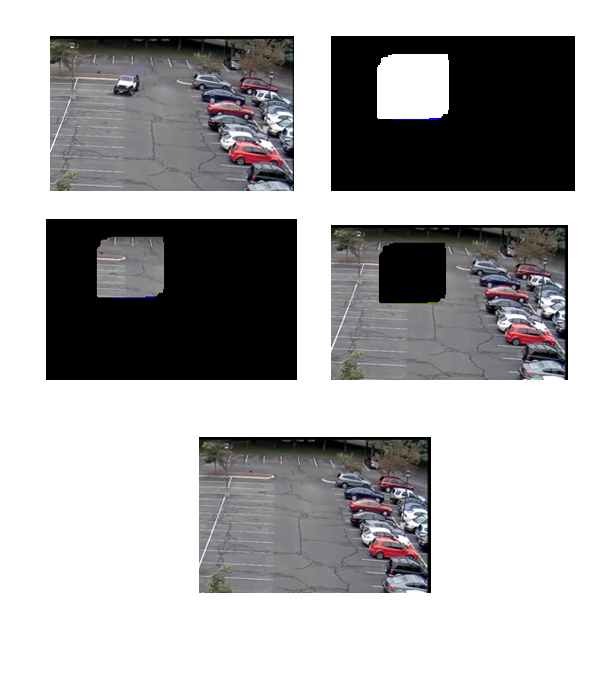
\includegraphics[width=1\textwidth]{FiguraFundo}
      \caption{Imagens representando o processo de geração do fundo dinâmico. No topo o quadro do vídeo e a máscara obtida. No centro a imagem do fundo anterior na região da máscara e a média entre os valores do quadro atual e do fundo anterior nos outros pontos e abaixo o fundo novo construído. }\label{fig:GeracaoFundo}
    \end{figure}

    A imagem de fundo obtida através do processo que foi descrito nessa seção é o objeto de estudo mais importante deste trabalho. Através dela são obtidas as informações relevantes para cumprir os objetivos desejados. Um objeto que aparece na imagem de fundo, é um objeto que parou de se mover e passou a ser um elemento estático do ambiente que está sendo filmado. No contexto do trabalho, isso significa que provavelmente um veículo estacionou. A região obtida pela subtração do fundo em momentos diferentes indica a posição de novos objetos estáticos. Esse processo é descrito na seçõa \ref{diferencasFundos}.





\section{Diferenças entre fundos} \label{diferencasFundos}

    Como foi mencionado ao final da seção \ref{geracaoFundo}, o programa identifica que um objeto que estava em movimento passou a estar parado quando este objeto aparece na imagem de fundo do vídeo. Analogamente, é possível identificar que um objeto que estava parado passou a se mover quando ele desaparece do \textit{background} dinâmico. Fica clara então a importância de se reconhecer quando elementos são adicionados ou removidos do fundo.

    Para identificar mudanças significativas na imagem de fundo do vídeo sendo observado, este programa utiliza o processo de subtração de imagens descrito na seção \ref{subtracao} com algumas modificações. A $t$ quadros do vídeo - onde $t$ é um valor determinado na etapa de calibração do sistema - o programa gera uma imagem de diferença entre o \textit{background} atual e o \textit{background} a $t$ quadros atrás. Essa imagem $Df$ de diferença é obtida através do mesmo processo utilizado para se obter a imagem $D$ de diferença entre dois \textit{frames} na seção \ref{segmentacaoVeiculos}. Essa imagem é submetida a um processo de fechamento, ou seja, a aplicação de uma erosão seguida de uma dilatação. Essa operação tem como objetivo uniformizar os contornos na imagem $Df$ e pricipalmente, eliminar manchas que são pequenas demais para serem consideradas. Por causa disso, a escolha do elemento estruturante para a erosão nessa etapa é muito importante. Esse elemento é o parâmetro que discerne entre os contornos relevantes e os irrelevantes em $Df$.

    Depois que os contornos que não são de interesse para o programa são eliminados de $Df$ é preciso submeter a imagem por um processo de limiarização para que ela seja compatível com as técnicas que serão aplicadas em seguida. Se a imagem do vídeo tem apenas um canal, o \textit{thresholding} aplicado é trivial, cada ponto que não é preto da imagem se torna branco, e os outros continuam pretos como antes. Quando o vídeo possue três canais, é preciso aplicar essa limiarização em cada canal e depois criar uma única imagem binária com as informações de cada canal através da operação lógica \textit{or}. Essa operação faz com que um determinado ponto da imagem resultando seja branco se o ponto de uma das duas imagens sendo operadas for branco e preto caso contrário. Ela é descrita pela equação \ref{equacaoOr}:


    \begin{equation}\label{equacaoOr}
       Or(x,y) = \left\{
        \begin{array}{l l}
        A(x,y) & \text{,A(x,y)=255} \\
        B(x,y) & \text{,B(x,y)=255}\\
        0 & \text{, A(x,y) = 0 e B(x,y) = 0} \\
         \end{array} \right.
     \end{equation}

     Onde $Or(x,y)$ é o valor do \textit{pixel} na posição $(x,y)$ da matriz resultante e $A(x,y)$ e $B(x,y)$ são os valores dos \textit{pixels} nas duas matrizes sobre as quais a operação está sendo aplicada.

     O resultado dessa operação sobre as imagens de binarizadas dos canais R,G e B dois a dois é uma imagem completamente preta, exceto por manchas brancas que representam regiões onde houve uma diferença entre os fundos nos dois momentos. Nessas regiões se pode assumir que ou um objeto novo se integrou ao fundo ou um objeto que antes fazia parte do \textit{background} deixou de fazer.

\section{Identificação de objetos no fundo} \label{identificacaoFundo}

    Apenas encontrar as regiões aonde houve uma diferença entre os fundos não é suficiente para atingir os objetivos do trabalho. Apesar destas regiões indicarem bem precisamente os locais da imagem onde um objeto apareceu ou desapareceu no fundo, elas não são capazes de fornecer algumas informações cruciais. Por exemplo, como saber se uma determinada mancha em $Df$ representa um novo objeto no fundo ou um carro que saiu de uma vaga aonde estava estacionado? Como determinar se o objeto que causou essa diferença sequer é um veículo? É preciso então voltar a analisar as informações contidas na imagem original do quadro do vídeo para identificar corretamente o que está acontecendo na região indicada. Dessa vez porém, o programa pode analisar apenas as pequenas regiões correspondentes àquelas em $Df$.

    Para responder a primeira pergunta apresentada no parágrafo anterior, o programa se utiliza de uma comparação de histogramas. Primeiramente é preciso extrair um histograma de uma região da imagem que seja suficientemente semelhante a uma vaga vazia. Esse histograma $H_{0}$ serve como um histograma de "controle", é o histograma que indica uma vaga vazia. É importante determinar $H_{0}$ de forma dinâmica, a fim de evitar que mudanças na iluminação do vídeo causem resultados incorretos. Para isso, o programa extrai esse histograma em intervalos de tempo regulares, de um espaço na imagem onde é sabido que não há carros. A determinação desse espaço pode ser feita manualmente no momento de instalação do programa ou posteriormente através de uma função de calibração. É importante escolher uma região onde ocorrem muito poucas mudanças na imagem de fundo e que seja semelhante ao fundo da imagem sem nenhum elemento. Em outras palavras, para o caso desse programa, deve-se escolher uma região que representa o chão do estacionamento e que não se espera que seja ocupada por objetos.

    Munido com $H_{0}$ o programa extrai o histograma $H_{1}$ da área do fundo atual correspondente à cada mancha branca presente em $Df$. Em seguida o histograma $H_{2}$ da mesma região no fundo a $t$ quadros atrás é extraído.  O programa faz uma comparação entre $H_{1}$ e $H_{2}$. Se os histograma forem suficientemente distintos, é considerado que houve uma mudança significativa no \textit{background}. Nesse caso, o programa compara $H_{1}$ e $H_{2}$ com $H_{0}$. Essa segunda comparação tem como objetivo determinar se um objeto foi adicionado ou removido do fundo. Quando o $H_{1}$ é semelhante a $H_{0}$, pode-se assumir que a região observada mostra uma vaga vazia. Por outro lado, quando $H_{2}$ é semelhante a $H_{0}$, é muito provável que a região observada mostra um objeto novo que se integrou ao fundo.

    Os histogramas são comparados através de um pequeno conjunto de parâmetros. Os parâmetros escolhidos não podem ser estritamente dependentes do tamanho da região analisada, já que não há garantia de que a região de controle terá o mesmo tamanho da região indicada em $Df$. O primeiro desses parâmetros é o nível de cinza que ocorre com mais frequência na região. Esse parâmetro é suficiente para determinar se as áreas analisadas são diferentes demais umas das outras, uma vez que imagens com níveis de cinza predominante demasiado diferentes certamente serão consideravelmente distintas. Porém, não se pode assumir o contrário, que uma coincidência nesse valor indica imagens semelhantes. Para complementar esse parâmetro o programa usa a técnica de intersecção detalhada na seção \ref{comparacaoHistogramas}. Se dois histogramas apresentam um valor muito alto de intersecção, é muito provável que essas duas imagens sejam parecidas.

    A figura \ref{DiferencaHistogramaFig} mostra esses dois histogramas para os dois momentos representados na figura \ref{SubtracaoFig}. Nela é visível a diferença da distribuição dos valores de cinza na imagem.


\begin{figure}
 \centering
\begin{subfigure}{.5\textwidth}
  \centering
  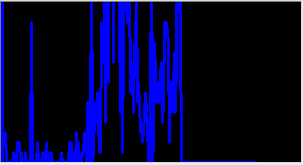
\includegraphics[width=.8\linewidth]{HistogramaFundo}
  \caption{}
  \label{DiferencaHistogramaFig:sfig1}
\end{subfigure}\


\begin{subfigure}{.5\textwidth}
  \centering
  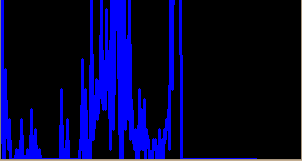
\includegraphics[width=.8\linewidth]{HistogramaFundoAnterior}
  \caption{}
  \label{DiferencaHistogramaFig:sfig2}
\end{subfigure}
\caption{(a) O histograma $H_{1}$ da figura \ref{Subtracao:sfig1} na área indicada por \ref{Subtracao:sfig3}; (b)O histograma $H_{2}$ da figura \ref{Subtracao:sfig2} na área indicada por \ref{Subtracao:sfig3}}
\label{DiferencaHistogramaFig}
\end{figure}

\section{Verificação de objetos no fundo}\label{verificaoObjetosFundo}

    Uma vez determinado que um objeto novo se integrou ao fundo da imagem, é preciso garantir então que o objeto que se integrou ao fundo na posição da vaga é realmente um veículo. O sistema não deve acusar que uma vaga foi ocupada quando algum outro corpo está sobre a vaga, como por exemplo uma pessoa que interrompeu seu trajeto sobre uma vaga ou a porta de um carro na vaga adjacente que ficou aberta por muito tempo. Observe que esse cuidado e suficiente para garantir que o sistema não libere vagas incorretamente quando um objeto que não é um carro sai dessa vaga, uma vez que a vaga nunca é marcada como ocupada nesse caso.

    Para identificar o objeto novo que apareceu no fundo da imagem, o sistema se utiliza pricipalmente de um recurso, a comparação da posição de um objeto identificado com os finais dos rastros identificados na seção \ref{rastreamentoVeiculos}. Antes de afirmar que uma vaga foi ocupada por um veículo quando identifica uma mudança no fundo sobre a área de uma vaga, o programa percorre o vetor de rastros obtidos e identifica se algum deles tem início em um ponto fora de qualquer vaga e o final dentro da região do objeto identificado. Se esse for o caso, garante-se que esse objeto que apareceu estava anteriormente em movimento. Isso significa que a diferença na região não foi causada por um objeto que surgiu subitamente na cena naquela posição, como um grande pico de ruído, uma porta que se abriu em um carro adjacente ou alguma mudança de cor sobre um carro parado, possivelmente causada por um vidro abrindo ou o reflexo de uma luz.

    Como um complemento a esse recurso, o programa se utiliza de um algoritmo simples de classificação para determinar a probabilidade de que o objeto seja de fato um carro. Esse algoritmo usa informações sobre as bordas presentes nas imagens para diferenciar principalmente veículos de pessoas. Características utilizadas para esse sistema de classificação incluem a largura, o comprimento, quanto uma determinada cor ocupa no objeto e a presença de alguns componentes como pára-brisas que ajudam a confirmar que o objeto é um veículo. Esse sistema será descrito com mais detalhes posteriormente.





